\documentclass[12pt,a4paper]{book}
\usepackage[utf8]{inputenc}									% Codificación
\usepackage[spanish,es-tabla]{babel}				% Lenguaje español, Tabla n: 
\usepackage[T1]{fontenc}										% Agregar fuentes con acentos
\usepackage{amsmath}												% Paquetes necesarios  para matemáticas
\usepackage{amsfonts}
\usepackage{amssymb}
\usepackage{makeidx}												% Paquete para indices
\usepackage{graphicx}												% Para manejar imagenes
\graphicspath{{imagenes/}}									% Ruta de las imagenes, solo escribir nombre de la imagen
%\usepackage[left=2cm,right=2cm,top=2cm,bottom=2cm]{geometry}
\usepackage[top=1in, left=0.9in, right=1.25in, bottom=1in]{geometry}		% Margenes
\author{Ciro Fabian Bermudez Marquez}
\title{Tesis}
\date{}
%-------------------------------------------------------------------------------
%                            Paquetes adicionales                              %
%-------------------------------------------------------------------------------
\input{librerias}
%-------------------------------------------------------------------------------
%                             Archivos a incluir                               %
%-------------------------------------------------------------------------------
\includeonly{
	portada,
	agradecimientos,
	ch1,
	ch2,
	ch3,
	Ap_A,
	Ap_B
}
%-------------------------------------------------------------------------------
%-------------------------------------------------------------------------------
\begin{document}
	\includepdf[pages=-]{portada3.pdf}
	\thispagestyle{empty}												% Limpiar estilos de pagina

\frontmatter
\onehalfspacing																% Desde este punto interlineado de 1.5
% 	\spacing{1.213}
	\chapter{Agradecimientos}

Agradezco a mi familia 

Agradezco al CONACYT ...

Agradezco a la Facultad de Ciencias de la Electrónica de la BUAP  ...

\pagestyle{normalstyle}												% Estilos de pagina personalizados
\tableofcontents            									% Genera el índice
\addcontentsline{toc}{chapter}{\contentsname}

\listoffigures              									% Indice de figuras
\listoftables               									% Indice de tablas
\lstlistoflistings

\mainmatter
	\chapter{Fundamentos teóricos}		

	Al igual que cuando se comienza a estudiar cálculo de orden entero, es necesario familiarizarse con la notación de los operadores matemáticos de la derivada y la integral. En la actualidad la notación más utilizada para el cálculo entero es la dada por Leibniz en (1686), donde el operador diferencial de n-ésimo orden esta definido como: $\frac{d^{n}}{dt^{n}}$, $D_{t}^{n}$ o simplemente $D^{n}$ con $n \in \mathbb{N}$. Utilizando el mismo razonamiento, puede definirse su operador inverso (antiderivada) de manera que el operador inverso de la derivada de n-ésimo orden está dado por: $_{a}D^{-n}_{t}$, donde $n \in \mathbb{N}$ y $a \in \mathbb{R}$ representa el límite inferior del dominio de la región donde se aplica dicho operador.
			
	Para generalizar el operador diferencial e integral para orden fraccionario se considera que este puede definirse para parámetros de orden real o incluso complejo. Esto implica que los operadores pueden definirse respectivamente como: $D^{\alpha}$ y $_{a}D^{\alpha}_{t}$ con $ \alpha \in \mathbb{R}$. 
		
	Es importante resaltar que no una hay una única definición de operadores diferencial fraccional ni integral sino varias expresiones definidas por diferentes autores, entre las mas usadas se encuentran la definición de Grünwald-Letnikov (GL), la de Riemann-Liouville (RL) y la de Caputo (Ca), cada una de estas con sus ventajas y desventajas desde el punto de vista del análisis matemático, complejidad computacional e implementación \cite{Petras2011}.
			
	\section{Definición de Grünwald-Letnikov}

	Comenzamos considerando que para el caso de orden entero la n-ésima derivada para una función $f$ con $n \in \mathbb{N}$ y $j>n$ esta dada por:
	\begin{equation}
		f^{(n)}(t) = \frac{d^{n}f}{dt^{n}} = \lim_{h \to 0 } \frac{1}{h^{n}} \sum_{j = 0}^{n} (-1)^{j} \binom{n}{j} f(t - jh)
		\label{ec:derivada_entera}
	\end{equation}
	donde $\binom{n}{j}$ representa el coeficiente binomial dado por la expresión:
			
	\begin{equation}
		\binom{n}{j} = \frac{n!}{j! (n-j)! } 
	\end{equation}
			
	Considerando valores negativos de $n$ tenemos:
	\begin{equation}
		\binom{-n}{j} = \frac{-n(-n-1)(-n-2) \cdots (-n -j +1 )}{j!}= (-1)^{j} \binomb{n}{j}
		\label{ec:binomio_n}
	\end{equation}
	donde $\binomb{n}{j}$ esta definido como:
			
	\begin{equation}
		\binomb{n}{j} = \frac{2(n+1) \cdots (n+j-1)}{j!}
	\end{equation}
	
		\subsection{Definición de derivada de Grünwald-Letnikov}
		
	Generalizando la ecuación (\ref{ec:derivada_entera}) podemos escribir la definición de derivada de orden fraccionario de orden  $\alpha$, ($\alpha \in \mathbb{R}$) como:
		
	\begin{equation}
		D^{\alpha}_{t} f(t) = \lim_{h \to 0} \frac{1}{h^{\alpha}}   \sum_{j = 0}^{\infty} (-1)^{j} \binom{\alpha}{j} f(t - jh)
		\label{ec:derivada_frac_GL}
	\end{equation}
			
	Para calcular el coeficiente binomial podemos utilizar la relación entre la función Gamma de Euler y el factorial definido como:
	\begin{equation}
		\binom{\alpha}{j}  = \frac{\alpha!}{j! (\alpha-j)!} = \frac{\Gamma (\alpha + 1)}{\Gamma(j+1) \Gamma(\alpha - j + 1)}
	\end{equation}
	donde la función Gamma de Euler con $r>0$ esta definida como:
			
	\begin{equation}
		\Gamma(r) = \int^{\infty}_{0} t^{r-1} e^{-t}dt
	\end{equation}
			
		\subsection{Definición de integral de Grünwald-Letnikov}
		
	Utilizando la ecuación (\ref{ec:derivada_frac_GL}) se puede definir un operador de tipo integral para la función $f$  sobre el dominio temporal $(a,t)$ considerando $n = \frac{t-a}{h}$ donde $a \in \mathbb{R}$ como:
			
	\begin{equation}
		_{a}D_{f}^{\alpha} = \lim_{h \to 0 } \frac{1}{h^{\alpha}} \sum_{j = 0}^{\left[ \frac{t-a}{h}  \right]} (-1)^{j} \binom{n}{j} f(t - jh)
	\end{equation}

		\subsection{Método numérico para la definición de GL}
		
	Utilizando como base la ecuación (\ref{ec:derivada_frac_GL}) esta se puede discretizar para los puntos $kh$, ($k = 1,2,\ldots$) de la siguiente manera:
			
	\begin{equation}
		_{\left( \frac{L_{m}}{h} \right)} D^{\alpha}_{t_{k}} f(t) \approx \frac{1}{h^{\alpha}} \sum_{j=0}^{k}(-1)^{j}  \binom{\alpha}{j} f(t_{k-j})
	\end{equation}
	donde $L_{m}$ es el tamaño de memoria (memory length), $t_{k} = kh$, $h$ es el paso de tiempo del cálculo y $(-1)^{j}\binom{\alpha}{j}$ son coeficientes binomiales $C_{j}^{(\alpha)}$ $(j=0,1,\ldots)$. Para su calculo utilizamos la siguiente expresión:
		
	\begin{equation}
		C_{0}^{(\alpha)} = 1, \qquad  C_{j}^{(\alpha)} = \left( 1 - \frac{1 + \alpha}{j} \right) C_{j-1}^{(\alpha)}
	\end{equation}
			
	Entonces, la solución numérica general de la ecuación diferencial fraccional:
		
	\begin{equation}
	 	_{a}D^{\alpha}_{t} y(t) = f(y(t), t)
	\end{equation}
	puede expresarse como:
		
	\begin{equation}
		y(t_{k}) = f(y(t_{k-1}), t_{k-1}) h^{\alpha} - \sum_{j=1}^{k} C_{j}^{(\alpha)} y(t_{k-j})
		\label{ec:GL_numerico}
	\end{equation}

	Para el termino de la memoria expresada por la sumatoria, el principio de memoria corta puede utilizarse. Entonces el indice superior de la sumatoria en la ecuación (\ref{ec:GL_numerico}) se cambiará por $\nu$ con las siguientes consideraciones: se usa $\nu = k$ para $k < \left( \frac{L_{m}}{h} \right)$ y $\nu = \left( \frac{L_{m}}{h} \right)$ para $k \geq (\frac{L_{m}}{h})$, o sin usar el principio de memoria corta se utiliza $\nu = k$ para toda $k$. 
	
	\section{Definición de Riemann-Liouville}
	
	Para esta definición consideramos la fórmula de Cauchy para la integral repetida que esta dada por:
	
	\begin{equation}
		f^{(-n)} (t) = \int_{a}^{t} \int_{a}^{\sigma_{1}}  \cdots \int_{a}^{\sigma_{n-1}} f(\sigma_{n}) d\sigma_{n} \cdots d\sigma_{2} d\sigma_{1} = \frac{1}{(n - 1)!} \int^{t}_{a} \frac{f(\tau)}{(t - \tau)^{1 - n}} d \tau
		\label{ec:cauchy}
	\end{equation}

		\subsection{Definición de integral de Riemann-Liouville}
		
	Utilizando las propiedades de la función Gamma de Euler con el factorial y la ecuación (\ref{ec:cauchy}) se puede escribir la definición de integral fraccionaria como:

	\begin{equation}
		_{a}D_{t}^{-\alpha} f(t) = \frac{1}{\Gamma( \alpha)} \int_{a}^{t} \frac{f(\tau)}{(t - \tau)^{ 1 - \alpha}} d \tau
		\label{ec:integral_RL}
	\end{equation}
	para $\alpha<0$ y $a \in \mathbb{R}$. No obstante para el caso de $0 < \alpha < 1$ y $f(t)$ siendo una función casual, esto es, $f(t)=0$ para $t<0$, la integral fraccionaria esta definida como:
	
	\begin{equation}
		_{0}D_{t}^{-\alpha} f(t) = \frac{1}{\Gamma( \alpha)} \int_{0}^{t} \frac{f(\tau)}{(t - \tau)^{ 1 - \alpha}} d \tau , \quad \mathrm{para} \quad 0 < \alpha < 1, \quad t > 0
	\end{equation}
		
		\subsection{Definición de derivada de Riemann-Liouville}
		
	De la ecuación (\ref{ec:integral_RL}) se puede escribir la definición de derivada fraccionaria de orden $\alpha$ de la siguiente manera:
	
	\begin{equation}
		_{a}D_{t}^{\alpha} f(t) = \frac{1}{\Gamma(n - \alpha)} \frac{d^{n}}{dt^{n}} \int_{a}^{t} \frac{f(\tau)}{(t - \tau)^{\alpha - n + 1}} d \tau
	\end{equation}
	donde $(n-1 < \alpha < n)$. Pero igual que con la integral si consideramos $0 < \alpha < 1$ y $f(t)$  una función casual, la derivada de orden fraccionaria se puede reescribir como:
	
	\begin{equation}
		_{0}D_{t}^{\alpha}f(t) = \frac{1}{\Gamma(n-\alpha)} \frac{d^{n}}{dt^{n}} \int_{0}^{t} \frac{f(\tau)}{(t - \tau)^{\alpha - n + 1}} d\tau
	\end{equation}
		
	\section{Transformada de Laplace de integrales y derivadas fraccionarias}
	
	La transformada de Laplace de la integral fraccionaria ya sea para Riemman-Liouville o para Grünwald-Letnikov esta definida como:
	
	\begin{equation}
	 	\mathcal{L} \{ _{0}D_{t}^{-p} f(t) \} = s^{-p} F(s)
	\end{equation} 
	y dadas condiciones iniciales cero  la transformada de Laplace de la derivada fraccionaria de orden $r$ para Grünwald-Letnikov, Riemann-Liouville y Caputo se reduce a:
	
	\begin{equation}
		\mathcal{L} \{ _{0}D_{t}^{r} f(t) \} = s^{r} F(s)
	\end{equation}
	
	
	\section{Expansión de fracciones continuas (CFE)}
	
	A una expresión de la forma:

	\begin{equation}
		a_{1} + \cfrac{b_{1}}{a_{2} + \cfrac{b_{2}}{a_{3} + \cfrac{b_{3}}{a_{4} + \genfrac{}{}{0pt}{0}{}{\ddots}}}}
		\label{ec:fracciones_cont}
	\end{equation} 
	se le conoce como una fracción continua. En general $a_{1},a_{2},a_{3}, \cdots, b_{1}, b_{2}, b_{3}$ pueden ser cualquier número real o complejo, y el número de términos pueden ser finito o infinito.

	Una manera más conveniente de escribir la ecuación (\ref{ec:fracciones_cont}) es:

	\begin{equation}
		a_{1} + \frac{b_{1}}{a_{2} } \genfrac{}{}{0pt}{0}{}{+}   \frac{b_{2}}{a_{3}}  \genfrac{}{}{0pt}{0}{}{+}  \frac{b_{3}}{a_{4}}  \genfrac{}{}{0pt}{0}{}{+}  \genfrac{}{}{0pt}{0}{}{\cdots} 
		\label{ec:fracciones_cont_sim}
	\end{equation}
	y es la que se encontrará normalmente en libros y artículos. Ambas notaciones son  muy similar y se puede pasar de una a otra sin mayor complicación.

	De la ecuación (\ref{ec:fracciones_cont_sim}) se pueden formar las siguientes fracciones:

	\begin{equation}
		c_{1} = \frac{a_{1}}{1} , \quad c_{2} = a_{1} + \frac{b_{1}}{a_{2}}, \quad c_{3} = a_{1} + \frac{b_{1}}{a_{2}} \genfrac{}{}{0pt}{0}{}{+} \frac{b_{2}}{a_{3}}, \quad \cdots
	\end{equation}
	las cuales se obtienen, en sucesión, de cortar el proceso de expansión después del primer, segundo, tercer, $\cdots$ término. Estas fracciones son llamadas primer, segundo, tercer, $\cdots$  convergente, respectivamente, de la fracción continua. El $n$-ésimo convergente es:

	\begin{equation}
		c_{n} = a_{1} + \frac{b_{1}}{a_{2}} \genfrac{}{}{0pt}{0}{}{+} \frac{b_{2}}{a_{3}} \genfrac{}{}{0pt}{0}{}{+} \genfrac{}{}{0pt}{0}{}{\cdots} \genfrac{}{}{0pt}{0}{}{+} \frac{b_{n-1}}{a_{n}}
	\end{equation}

	En 1776 Lagrange obtuvo la expansión de fracciones continuas (CFE) para la ecuación $(1 + x)^{\alpha}$ como se muestra a continuación \cite{Olds2009}:

	\begin{equation}
 		(1 + x)^{\alpha} = \cfrac{1}{1 - \cfrac{\alpha x}{1 + \cfrac{\cfrac{1(1 + \alpha)}{1\cdot2}\,x}{1 + \cfrac{\cfrac{1(1 - \alpha)}{2\cdot3}\,x}{1 + \cfrac{\cfrac{2(2 + \alpha)}{3\cdot4}\,x}{1 + \cfrac{\cfrac{2(2 - k)}{4\cdot5}\,x}{1 + \cfrac{\cfrac{3(3 + \alpha)}{5\cdot6}\,x}{1 + \genfrac{}{}{0pt}{0}{}{\ddots}}}}}}}}
		 \label{ec:lagrange}
	\end{equation}
	y escrita de una manera más compacta:

	\begin{equation}
 		(1 + x)^{\alpha} = \frac{1}{1} \genfrac{}{}{0pt}{0}{}{-} \frac{\alpha x}{1} \genfrac{}{}{0pt}{0}{}{+} \frac{\frac{1(1 + \alpha)}{1\cdot2}\,x}{1} \genfrac{}{}{0pt}{0}{}{+} \frac{\frac{1(1 - \alpha)}{2\cdot3}\,x}{1} \genfrac{}{}{0pt}{0}{}{+} \frac{\frac{2(2 + \alpha)}{3\cdot4}\,x}{1} \genfrac{}{}{0pt}{0}{}{+} \frac{\frac{2(2 - \alpha)}{4\cdot5}\,x}{1} \genfrac{}{}{0pt}{0}{}{+} \genfrac{}{}{0pt}{0}{}{\cdots} 
		\label{ec:lagrange_conv}
	\end{equation}
	la ecuación (\ref{ec:lagrange_conv}) puede reescribirse convenientemente multiplicando un $m$ en el numerador y en el denominador como se muestra a continuación:

	\begin{equation}
 		(1 + x)^{\alpha} = \frac{1}{1} \genfrac{}{}{0pt}{0}{}{-} \frac{\alpha x}{1} \genfrac{}{}{0pt}{0}{}{+}  \frac{ {\color{red} 2} \cdot \frac{1(1 + \alpha)}{1\cdot2}\,x}{{\color{red} 2} \cdot 1} \genfrac{}{}{0pt}{0}{}{+} \frac{ {\color{blue} 3} \cdot {\color{red} 2} \cdot \frac{1(1 - \alpha)}{2\cdot3}\,x}{{\color{blue} 3} \cdot 1} \genfrac{}{}{0pt}{0}{}{+} \frac{{\color{blue} 3} \cdot \frac{2(2 + \alpha)}{3\cdot4}\,x}{1}   \genfrac{}{}{0pt}{0}{}{+} \genfrac{}{}{0pt}{0}{}{\cdots} 
	\end{equation}
	hay que notar que cada denominador esta compuesto por 2 términos, esto se puede ver claramente en la ecuación (\ref{ec:lagrange}), y que contando el término del numerador, $m$ se tiene que agregar en 3 lugares distintos. Si se eligen $m_{1} = 2$, $m_{2} = 3$, $m_{3} = 2$, $\ldots$ de manera que se simplifique la ecuación obtenemos:

	\begin{equation}
 		(1 + x)^{\alpha} = \frac{1}{1}  \genfrac{}{}{0pt}{0}{}{-} \frac{\alpha x}{1} \genfrac{}{}{0pt}{0}{}{+} \frac{(1 + \alpha)x}{2} \genfrac{}{}{0pt}{0}{}{+} \frac{(1 - \alpha)x}{3} \genfrac{}{}{0pt}{0}{}{+} \frac{(2 + \alpha)x}{2} \genfrac{}{}{0pt}{0}{}{+} \frac{(2-\alpha)x}{5} \genfrac{}{}{0pt}{0}{}{+} \genfrac{}{}{0pt}{0}{}{\cdots}
 		\label{ec:cfe_inutil}
	\end{equation}

	La ecuación (\ref{ec:cfe_inutil}) se puede encontrar en distintos artículos \cite{Krishna2008,Krishna2011}, no obstante para programar un algoritmo que obtenga la aproximación de $(1 + x)^{\alpha}$ hasta el $n$-ésimo convergente resulta poco intuitiva. Para este fin la ecuación (\ref{ec:lagrange_conv}) resulta más sencilla y contiene un patrón que puede explotarse.

	El $n$-ésimo término de la expansión de fracciones continuas para la ecuación (\ref{ec:lagrange_conv}) se puede calcular utilizando la siguiente ecuación:

	\begin{equation}
		\frac{\psi(n) \left[ \psi(n) + (-1)^{n} \alpha \right]}{(n-1)n}
		\label{ec:calculo_terminos_cfe}
	\end{equation}
	donde la función $\psi(x)$ para $x\geq2$, $x\in \mathbb{Z}^{+}$ esta definida como\footnote{$\left\lfloor x\right\rfloor$ es  la función redondeo hacia el entero inferior anterior.}:

	\begin{equation}
		\psi(x) = \left\lfloor \frac{x}{2}\right\rfloor
	\end{equation}

	La ecuación (\ref{ec:calculo_terminos_cfe}) se puede utilizar de manera recursiva desde el $n$-ésimo término hasta el segundo sin olvidar que cada uno de estos siempre debe ir acompañado de la suma de un uno. También vale la pena resaltar que el primer término de la expansión es $\cfrac{1}{1} \genfrac{}{}{0pt}{0}{}{-} \cfrac{\alpha x}{1}$ en conjunto. 

	Sustituyendo $x = s - 1$ y limitando el número de términos de la ecuación (\ref{ec:lagrange_conv}) obtenemos la aproximación racional para $s^{\alpha}$ y para obtener la aproximación racional de $\frac{1}{s^{\alpha}}$ la expresión tiene que ser simplemente invertida. En el apéndice \ref{cod:cfetf} se muestra un programa en MATLAB que calcula la aproximación para un integrador fraccionario de orden $\alpha$ eligiendo el número de términos $n$, utilizando el método de CFE descrito previamente.

	En general la aproximación utilizando la CFE para un integrador fraccionario $\frac{1}{s^{\alpha}}$ utilizando los primeros dos términos resulta en una función de transferencia de primer orden como se muestra a continuación:

	\begin{equation}
		\genfrac{}{}{0pt}{0}{}{_{(c_{2})}} \frac{1}{s^{\alpha}} \approx \frac{(1 - \alpha)s + (1 + \alpha) }{(1 + \alpha)s + (1 - \alpha)} 
	\end{equation}

	Al utilizar un número impar de términos el grado del numerador de la función de transferencia siempre será mayor en uno al del denominador, además de que el coeficiente de mayor grado del numerador siempre tendrá signo negativo, esto resulta problemático en la implementación y debido a estas observaciones es recomendable solo trabajar con un número par de términos.

	La aproximación de segundo orden tiene la forma:

	\begin{equation}
		\genfrac{}{}{0pt}{0}{}{_{(c_{4})}} \frac{1}{s^{\alpha}} \approx \frac{(\alpha^{2} - 3\alpha + 2) s^{2} + (8 - 2 \alpha^{2})s + (\alpha^{2} + 3\alpha + 2) }{(\alpha^{2} + 3\alpha + 2) s^{2} + (8 - 2 \alpha^{2})s + (\alpha^{2} - 3\alpha + 2)}
	\end{equation}

	La ventaja de utilizar la aproximación de CFE es que convertimos el problema de orden fraccionario a uno de orden entero de manera sistemática. Por ejemplo para un integrador de orden fraccionario $\alpha = 0.5$ sus aproximaciones son las mostradas en la Tabla \ref{tab:aprox_cfe_alpha_0.5} y su diagrama de bode es el mostrado en la Figura .


	\begin{table}[!hbp]
		\caption{Aproximación racional de $\frac{1}{s^{0.5}}$}
		\label{tab:aprox_cfe_alpha_0.5}
		\centering
%		\resizebox{\textwidth}{!}{
		\begin{tabular}{c c c}
			\hline
			\textbf{Orden} &  \textbf{No. de términos} & \textbf{Aproximación racional}\\
			\hline
			$1$ 		& $2$ 		&  $\cfrac{s + 3}{3s + 1}$\\
					 		& 		 		& \\
			$2$			& $4$ 		&  $\cfrac{s^{2} + 10s + 5}{5 s^{2} + 10s + 1}$\\
							& 		 		& \\
			$3$ 		& $6$ 		&  $\cfrac{s^{3} + 21s^{2} + 35s + 7}{7 s^3 + 35 s^2 + 21 s + 1}$	\\
							& 		 		& \\
			$4$ 		& $8$ 		&  $\cfrac{s^4 + 36 s^3 + 126 s^2 + 84 s + 9}{9 s^4 + 84 s^3 + 126 s^2 + 36 s + 1}$\\
							& 		 		& \\
			$5$ 		& $10$ 		&  $\cfrac{s^5 + 55 s^4 + 330 s^3 + 462 s^2 + 165 s + 11}{11 s^5 + 165 s^4 + 462 s^3 + 330 s^2 + 55 s + 1}$\\
							& 		 		& \\
			\hline
		\end{tabular}
%		}
	\end{table}
	
	Esto es una prueba para ver si funciona bien o no

	
	\chapter{Fundamentos teóricos}		

	Cuando se comienza a estudiar cálculo de orden entero es necesario familiarizarse con la notación de los operadores matemáticos de la derivada y la integral, con el cálculo fraccionario ocurre lo mismo. En la actualidad la notación más utilizada para el cálculo entero es la dada por Leibniz en (1686), donde el operador diferencial de n-ésimo orden esta definido como: $\frac{d^{n}}{dt^{n}}$, $D_{t}^{n}$ o simplemente $D^{n}$ con $n \in \mathbb{N}$. Utilizando el mismo razonamiento, puede definirse su operador inverso (antiderivada) de manera que el operador inverso de la derivada de n-ésimo orden está dado por: $_{a}D^{-n}_{t}$, donde $n \in \mathbb{N}$ y $a \in \mathbb{R}$ representa el límite inferior del dominio de la región donde se aplica dicho operador.
			
	Para generalizar el operador diferencial e integral para orden fraccionario se considera que este puede definirse para parámetros de orden real o incluso complejo. Esto implica que los operadores pueden definirse respectivamente como: $D^{\alpha}$ y $_{a}D^{\alpha}_{t}$ con $ \alpha \in \mathbb{R}$. 
		
	Es importante tener presente que no una hay una única definición para los operadores diferencial e integral fraccional, sino varias expresiones definidas por diferentes autores, entre las mas usadas se encuentran la definición de Grünwald-Letnikov (GL), la de Riemann-Liouville (RL) y la de Caputo (Ca), cada una de estas con sus ventajas y desventajas desde el punto de vista del análisis matemático, complejidad computacional e implementación \cite{Petras2011}.
			
	\section{Definición de Grünwald-Letnikov}

	Comenzamos considerando que para el caso de orden entero la n-ésima derivada para una función $f$ con $n \in \mathbb{N}$ y $j>n$ esta dada por:
	\begin{equation}
		f^{(n)}(t) = \frac{d^{n}f}{dt^{n}} = \lim_{h \to 0 } \frac{1}{h^{n}} \sum_{j = 0}^{n} (-1)^{j} \binom{n}{j} f(t - jh)
		\label{ec:derivada_entera}
	\end{equation}
	donde $\binom{n}{j}$ representa el coeficiente binomial dado por la expresión:
			
	\begin{equation}
		\binom{n}{j} = \frac{n!}{j! (n-j)! } 
	\end{equation}
	considerando valores negativos de $n$ tenemos:
	\begin{equation}
		\binom{-n}{j} = \frac{-n(-n-1)(-n-2) \cdots (-n -j +1 )}{j!}= (-1)^{j} \binomb{n}{j}
		\label{ec:binomio_n}
	\end{equation}
	donde $\binomb{n}{j}$ esta definido como:
			
	\begin{equation}
		\binomb{n}{j} = \frac{2(n+1) \cdots (n+j-1)}{j!}
	\end{equation}
	
		\subsection{Definición de derivada de Grünwald-Letnikov}
		
	Generalizando la ecuación (\ref{ec:derivada_entera}) podemos escribir la definición de derivada de orden fraccionario de orden  $\alpha$, ($\alpha \in \mathbb{R}$) como:
		
	\begin{equation}
		D^{\alpha}_{t} f(t) = \lim_{h \to 0} \frac{1}{h^{\alpha}}   \sum_{j = 0}^{\infty} (-1)^{j} \binom{\alpha}{j} f(t - jh)
		\label{ec:derivada_frac_GL}
	\end{equation}
	para calcular el coeficiente binomial podemos utilizar la relación entre la función Gamma de Euler y el factorial definido como:
	\begin{equation}
		\binom{\alpha}{j}  = \frac{\alpha!}{j! (\alpha-j)!} = \frac{\Gamma (\alpha + 1)}{\Gamma(j+1) \Gamma(\alpha - j + 1)}
	\end{equation}
	donde la función Gamma de Euler con $r>0$ esta definida como:
			
	\begin{equation}
		\Gamma(r) = \int^{\infty}_{0} t^{r-1} e^{-t}dt
	\end{equation}
			
		\subsection{Definición de integral de Grünwald-Letnikov}
		
	Utilizando la ecuación (\ref{ec:derivada_frac_GL}) se puede definir un operador de tipo integral para la función $f$  sobre el dominio temporal $(a,t)$ considerando $n = \frac{t-a}{h}$ donde $a \in \mathbb{R}$ como:
			
	\begin{equation}
		_{a}D_{f}^{\alpha} = \lim_{h \to 0 } \frac{1}{h^{\alpha}} \sum_{j = 0}^{\left[ \frac{t-a}{h}  \right]} (-1)^{j} \binom{n}{j} f(t - jh)
	\end{equation}

		\subsection{Método numérico para la definición de GL}
		
	Utilizando como base la ecuación (\ref{ec:derivada_frac_GL}) esta se puede discretizar para los puntos $kh$, ($k = 1,2,\ldots$) de la siguiente manera:
			
	\begin{equation}
		_{\left( \frac{L_{m}}{h} \right)} D^{\alpha}_{t_{k}} f(t) \approx \frac{1}{h^{\alpha}} \sum_{j=0}^{k}(-1)^{j}  \binom{\alpha}{j} f(t_{k-j})
	\end{equation}
	donde $L_{m}$ es el tamaño de memoria (memory length), $t_{k} = kh$, $h$ es el paso de tiempo del cálculo y $(-1)^{j}\binom{\alpha}{j}$ son coeficientes binomiales $C_{j}^{(\alpha)}$ $(j=0,1,\ldots)$. Para su calculo utilizamos la siguiente expresión:
		
	\begin{equation}
		C_{0}^{(\alpha)} = 1, \qquad  C_{j}^{(\alpha)} = \left( 1 - \frac{1 + \alpha}{j} \right) C_{j-1}^{(\alpha)}
	\end{equation}
			
	Entonces, la solución numérica general de la ecuación diferencial fraccional:
		
	\begin{equation}
	 	_{a}D^{\alpha}_{t} y(t) = f(y(t), t)
	\end{equation}
	puede expresarse como:
		
	\begin{equation}
		y(t_{k}) = f(y(t_{k-1}), t_{k-1}) h^{\alpha} - \sum_{j=1}^{k} C_{j}^{(\alpha)} y(t_{k-j})
		\label{ec:GL_numerico}
	\end{equation}

	Para el termino de la memoria expresada por la sumatoria, el principio de memoria corta puede utilizarse. Entonces el indice superior de la sumatoria en la ecuación (\ref{ec:GL_numerico}) se cambiará por $\nu$ con las siguientes consideraciones: se usa $\nu = k$ para $k < \left( \frac{L_{m}}{h} \right)$ y $\nu = \left( \frac{L_{m}}{h} \right)$ para $k \geq (\frac{L_{m}}{h})$, o sin usar el principio de memoria corta se utiliza $\nu = k$ para toda $k$. 
	
	\section{Definición de Riemann-Liouville}
	
	Para esta definición consideramos la fórmula de Cauchy para la integral repetida que esta dada por:
	
	\begin{equation}
		f^{(-n)} (t) = \int_{a}^{t} \int_{a}^{\sigma_{1}}  \cdots \int_{a}^{\sigma_{n-1}} f(\sigma_{n}) d\sigma_{n} \cdots d\sigma_{2} d\sigma_{1} = \frac{1}{(n - 1)!} \int^{t}_{a} \frac{f(\tau)}{(t - \tau)^{1 - n}} d \tau
		\label{ec:cauchy}
	\end{equation}

		\subsection{Definición de integral de Riemann-Liouville}
		
	Utilizando las propiedades de la función Gamma de Euler con el factorial y la ecuación (\ref{ec:cauchy}) se puede escribir la definición de integral fraccionaria como:

	\begin{equation}
		_{a}D_{t}^{-\alpha} f(t) = \frac{1}{\Gamma( \alpha)} \int_{a}^{t} \frac{f(\tau)}{(t - \tau)^{ 1 - \alpha}} d \tau
		\label{ec:integral_RL}
	\end{equation}
	para $\alpha<0$ y $a \in \mathbb{R}$. No obstante para el caso de $0 < \alpha < 1$ y $f(t)$ siendo una función casual, esto es, $f(t)=0$ para $t<0$, la integral fraccionaria esta definida como:
	
	\begin{equation}
		_{0}D_{t}^{-\alpha} f(t) = \frac{1}{\Gamma( \alpha)} \int_{0}^{t} \frac{f(\tau)}{(t - \tau)^{ 1 - \alpha}} d \tau , \quad \mathrm{para} \quad 0 < \alpha < 1, \quad t > 0
	\end{equation}
		
		\subsection{Definición de derivada de Riemann-Liouville}
		
	De la ecuación (\ref{ec:integral_RL}) se puede escribir la definición de derivada fraccionaria de orden $\alpha$ de la siguiente manera:
	
	\begin{equation}
		_{a}D_{t}^{\alpha} f(t) = \frac{1}{\Gamma(n - \alpha)} \frac{d^{n}}{dt^{n}} \int_{a}^{t} \frac{f(\tau)}{(t - \tau)^{\alpha - n + 1}} d \tau
	\end{equation}
	donde $(n-1 < \alpha < n)$. Pero igual que con la integral si consideramos $0 < \alpha < 1$ y $f(t)$  una función casual, la derivada de orden fraccionaria se puede reescribir como:
	
	\begin{equation}
		_{0}D_{t}^{\alpha}f(t) = \frac{1}{\Gamma(n-\alpha)} \frac{d^{n}}{dt^{n}} \int_{0}^{t} \frac{f(\tau)}{(t - \tau)^{\alpha - n + 1}} d\tau
	\end{equation}
		
	\section{Transformada de Laplace de integrales y derivadas fraccionarias}
	
	La transformada de Laplace de la integral fraccionaria ya sea para Riemman-Liouville o para Grünwald-Letnikov esta definida como:
	
	\begin{equation}
	 	\mathcal{L} \{ _{0}D_{t}^{-p} f(t) \} = s^{-p} F(s)
	\end{equation} 
	y dadas condiciones iniciales cero  la transformada de Laplace de la derivada fraccionaria de orden $r$ para Grünwald-Letnikov, Riemann-Liouville y Caputo se reduce a:
	
	\begin{equation}
		\mathcal{L} \{ _{0}D_{t}^{r} f(t) \} = s^{r} F(s)
	\end{equation}
	
	
	\section{Expansión de fracciones continuas (CFE)}
	
	A una expresión de la forma:

	\begin{equation}
		a_{1} + \cfrac{b_{1}}{a_{2} + \cfrac{b_{2}}{a_{3} + \cfrac{b_{3}}{a_{4} + \genfrac{}{}{0pt}{0}{}{\ddots}}}}
		\label{ec:fracciones_cont}
	\end{equation} 
	se le conoce como una fracción continua. En general $a_{1},a_{2},a_{3}, \cdots, b_{1}, b_{2}, b_{3}$ pueden ser cualquier número real o complejo, y el número de términos pueden ser finito o infinito.

	Una manera más conveniente de escribir la ecuación (\ref{ec:fracciones_cont}) es:

	\begin{equation}
		a_{1} + \frac{b_{1}}{a_{2} } \genfrac{}{}{0pt}{0}{}{+}   \frac{b_{2}}{a_{3}}  \genfrac{}{}{0pt}{0}{}{+}  \frac{b_{3}}{a_{4}}  \genfrac{}{}{0pt}{0}{}{+}  \genfrac{}{}{0pt}{0}{}{\cdots} 
		\label{ec:fracciones_cont_sim}
	\end{equation}
	y es la que se encontrará normalmente en libros y artículos. Ambas notaciones son  muy similares y se puede pasar de una a otra sin mayor complicación.

	De la ecuación (\ref{ec:fracciones_cont_sim}) se pueden formar las siguientes fracciones:

	\begin{equation}
		c_{1} = \frac{a_{1}}{1} , \quad c_{2} = a_{1} + \frac{b_{1}}{a_{2}}, \quad c_{3} = a_{1} + \frac{b_{1}}{a_{2}} \genfrac{}{}{0pt}{0}{}{+} \frac{b_{2}}{a_{3}}, \quad \cdots
	\end{equation}
	las cuales se obtienen, en sucesión, de cortar el proceso de expansión después del primer, segundo, tercer, $\cdots$ término. Estas fracciones son llamadas primer, segundo, tercer, $\cdots$  convergente, respectivamente, de la fracción continua. El $n$-ésimo convergente es:

	\begin{equation}
		c_{n} = a_{1} + \frac{b_{1}}{a_{2}} \genfrac{}{}{0pt}{0}{}{+} \frac{b_{2}}{a_{3}} \genfrac{}{}{0pt}{0}{}{+} \genfrac{}{}{0pt}{0}{}{\cdots} \genfrac{}{}{0pt}{0}{}{+} \frac{b_{n-1}}{a_{n}}
	\end{equation}

	En 1776 Lagrange obtuvo la expansión de fracciones continuas (CFE) para la ecuación $(1 + x)^{\alpha}$ como se muestra a continuación \cite{Olds2009}:

	\begin{equation}
 		(1 + x)^{\alpha} = \cfrac{1}{1 - \cfrac{\alpha x}{1 + \cfrac{\cfrac{1(1 + \alpha)}{1\cdot2}\,x}{1 + \cfrac{\cfrac{1(1 - \alpha)}{2\cdot3}\,x}{1 + \cfrac{\cfrac{2(2 + \alpha)}{3\cdot4}\,x}{1 + \cfrac{\cfrac{2(2 - k)}{4\cdot5}\,x}{1 + \cfrac{\cfrac{3(3 + \alpha)}{5\cdot6}\,x}{1 + \genfrac{}{}{0pt}{0}{}{\ddots}}}}}}}}
		 \label{ec:lagrange}
	\end{equation}
	y escrita de una manera más compacta:

	\begin{equation}
 		(1 + x)^{\alpha} = \frac{1}{1} \genfrac{}{}{0pt}{0}{}{-} \frac{\alpha x}{1} \genfrac{}{}{0pt}{0}{}{+} \frac{\frac{1(1 + \alpha)}{1\cdot2}\,x}{1} \genfrac{}{}{0pt}{0}{}{+} \frac{\frac{1(1 - \alpha)}{2\cdot3}\,x}{1} \genfrac{}{}{0pt}{0}{}{+} \frac{\frac{2(2 + \alpha)}{3\cdot4}\,x}{1} \genfrac{}{}{0pt}{0}{}{+} \frac{\frac{2(2 - \alpha)}{4\cdot5}\,x}{1} \genfrac{}{}{0pt}{0}{}{+} \genfrac{}{}{0pt}{0}{}{\cdots} 
		\label{ec:lagrange_conv}
	\end{equation}
	la ecuación (\ref{ec:lagrange_conv}) puede reescribirse convenientemente multiplicando un $m$ en el numerador y en el denominador como se muestra a continuación:

	\begin{equation}
 		(1 + x)^{\alpha} = \frac{1}{1} \genfrac{}{}{0pt}{0}{}{-} \frac{\alpha x}{1} \genfrac{}{}{0pt}{0}{}{+}  \frac{ {\color{red} 2} \cdot \frac{1(1 + \alpha)}{1\cdot2}\,x}{{\color{red} 2} \cdot 1} \genfrac{}{}{0pt}{0}{}{+} \frac{ {\color{blue} 3} \cdot {\color{red} 2} \cdot \frac{1(1 - \alpha)}{2\cdot3}\,x}{{\color{blue} 3} \cdot 1} \genfrac{}{}{0pt}{0}{}{+} \frac{{\color{blue} 3} \cdot \frac{2(2 + \alpha)}{3\cdot4}\,x}{1}   \genfrac{}{}{0pt}{0}{}{+} \genfrac{}{}{0pt}{0}{}{\cdots} 
	\end{equation}
	hay que notar que cada denominador esta compuesto por 2 términos, esto se puede ver claramente en la ecuación (\ref{ec:lagrange}), y que contando el término del numerador, $m$ se tiene que agregar en 3 lugares distintos. Si se eligen $m_{1} = 2$, $m_{2} = 3$, $m_{3} = 2$, $\ldots$ de manera que se simplifique la ecuación obtenemos:

	\begin{equation}
 		(1 + x)^{\alpha} = \frac{1}{1}  \genfrac{}{}{0pt}{0}{}{-} \frac{\alpha x}{1} \genfrac{}{}{0pt}{0}{}{+} \frac{(1 + \alpha)x}{2} \genfrac{}{}{0pt}{0}{}{+} \frac{(1 - \alpha)x}{3} \genfrac{}{}{0pt}{0}{}{+} \frac{(2 + \alpha)x}{2} \genfrac{}{}{0pt}{0}{}{+} \frac{(2-\alpha)x}{5} \genfrac{}{}{0pt}{0}{}{+} \genfrac{}{}{0pt}{0}{}{\cdots}
 		\label{ec:cfe_inutil}
	\end{equation}

	La ecuación (\ref{ec:cfe_inutil}) se puede encontrar en distintos artículos \cite{Krishna2008,Krishna2011}, no obstante para programar un algoritmo que obtenga la aproximación de $(1 + x)^{\alpha}$ hasta el $n$-ésimo convergente resulta poco intuitiva. Para este fin la ecuación (\ref{ec:lagrange_conv}) resulta más sencilla y contiene un patrón que puede explotarse.

	El $n$-ésimo término de la expansión de fracciones continuas para la ecuación (\ref{ec:lagrange_conv}) se puede calcular utilizando la siguiente ecuación:

	\begin{equation}
		\frac{\psi(n) \left[ \psi(n) + (-1)^{n} \alpha \right]}{(n-1)n}
		\label{ec:calculo_terminos_cfe}
	\end{equation}
	donde la función $\psi(x)$ para $x\geq2$, $x\in \mathbb{Z}^{+}$ esta definida como\footnote{$\left\lfloor x\right\rfloor$ es  la función redondeo hacia el entero inferior anterior.}:

	\begin{equation}
		\psi(x) = \left\lfloor \frac{x}{2}\right\rfloor
	\end{equation}

	La ecuación (\ref{ec:calculo_terminos_cfe}) se puede utilizar de manera recursiva desde el $n$-ésimo término hasta el segundo sin olvidar que a cada término se le debe sumar un uno. También vale la pena resaltar que el primer término de la expansión es $\cfrac{1}{1} \genfrac{}{}{0pt}{0}{}{-} \cfrac{\alpha x}{1}$ . 

	Sustituyendo $x = s - 1$ y limitando el número de términos de la ecuación (\ref{ec:lagrange_conv}) obtenemos la aproximación racional para $s^{\alpha}$ y para obtener la aproximación racional de $\frac{1}{s^{\alpha}}$ la expresión tiene que ser simplemente invertida. En el apéndice \ref{cod:cfetf} se encuentra un programa escrito en MATLAB que calcula la aproximación para un integrador fraccionario de orden $\alpha$ eligiendo el número de términos $n$ utilizando el método de CFE descrito previamente.

	En general la aproximación utilizando la CFE para un integrador fraccionario $\frac{1}{s^{\alpha}}$ utilizando los primeros dos términos resulta en una función de transferencia de primer orden como se muestra a continuación:

	\begin{equation}
		\genfrac{}{}{0pt}{0}{}{_{(c_{2})}} \frac{1}{s^{\alpha}} \approx \frac{(1 - \alpha)s + (1 + \alpha) }{(1 + \alpha)s + (1 - \alpha)} 
	\end{equation}

	Al utilizar un número impar de términos el grado del numerador de la función de transferencia siempre será mayor en uno al del denominador, además de que el coeficiente de mayor grado del numerador siempre tendrá signo negativo, esto resulta problemático en la implementación y debido a estas observaciones es recomendable solo trabajar con un número par de términos.

	La aproximación de segundo orden tiene la forma:

	\begin{equation}
		\genfrac{}{}{0pt}{0}{}{_{(c_{4})}} \frac{1}{s^{\alpha}} \approx \frac{(\alpha^{2} - 3\alpha + 2) s^{2} + (8 - 2 \alpha^{2})s + (\alpha^{2} + 3\alpha + 2) }{(\alpha^{2} + 3\alpha + 2) s^{2} + (8 - 2 \alpha^{2})s + (\alpha^{2} - 3\alpha + 2)}
	\end{equation}
	la ventaja de utilizar la aproximación de CFE es que convertimos el problema de orden fraccionario a uno de orden entero de manera sistemática. Tomemos como ejemplo un integrador de orden fraccionario con $\alpha = 0.5$, sus aproximaciones son las mostradas en la Tabla \ref{tab:aprox_cfe_alpha_0.5} y sus correspondientes diagramas de bode se muestran en la Figura \ref{fig:F1_bode_integrador_alpha05}.


	\begin{table}[!hbp]
		\caption{Aproximaciones racionales de $\frac{1}{s^{0.5}}$}
		\label{tab:aprox_cfe_alpha_0.5}
		\centering
%		\resizebox{\textwidth}{!}{
		\begin{tabular}{c c c}
			\hline
			\textbf{Orden} &  \textbf{No. de términos} & \textbf{Aproximación racional}\\
			\hline
			$1$ 		& $2$ 		&  $\cfrac{s + 3}{3s + 1}$\\
					 		& 		 		& \\
			$2$			& $4$ 		&  $\cfrac{s^{2} + 10s + 5}{5 s^{2} + 10s + 1}$\\
							& 		 		& \\
			$3$ 		& $6$ 		&  $\cfrac{s^{3} + 21s^{2} + 35s + 7}{7 s^3 + 35 s^2 + 21 s + 1}$	\\
							& 		 		& \\
			$4$ 		& $8$ 		&  $\cfrac{s^4 + 36 s^3 + 126 s^2 + 84 s + 9}{9 s^4 + 84 s^3 + 126 s^2 + 36 s + 1}$\\
							& 		 		& \\
			$5$ 		& $10$ 		&  $\cfrac{s^5 + 55 s^4 + 330 s^3 + 462 s^2 + 165 s + 11}{11 s^5 + 165 s^4 + 462 s^3 + 330 s^2 + 55 s + 1}$\\
							& 		 		& \\
			\hline
		\end{tabular}
%		}
	\end{table}
	
	Analizando la Figura \ref{fig:F1_bode_integrador_alpha05} se puede resaltar que en general la aproximación aumenta su ancho de banda conforme el orden de la función de transferencia aumenta y que de mismo modo el error con respecto al integrador ideal disminuye, lo cual era de esperarse, el ancho de banda útil es de $10^{-1}$ rad/s hasta $10^{1}$ rad/s, es decir aproximadamente dos décadas, no obstante un análisis más profundo es necesario para notar otras peculiaridades que ocurren en este tipo de aproximaciones.
	
	\begin{figure}[hbtp]
		\caption{Diagramas de bode comparativos de integrador fraccionario $\alpha = 0.5$, funciones de transferencia de primer hasta quito orden.} 
		\label{fig:F1_bode_integrador_alpha05}
		\centering
		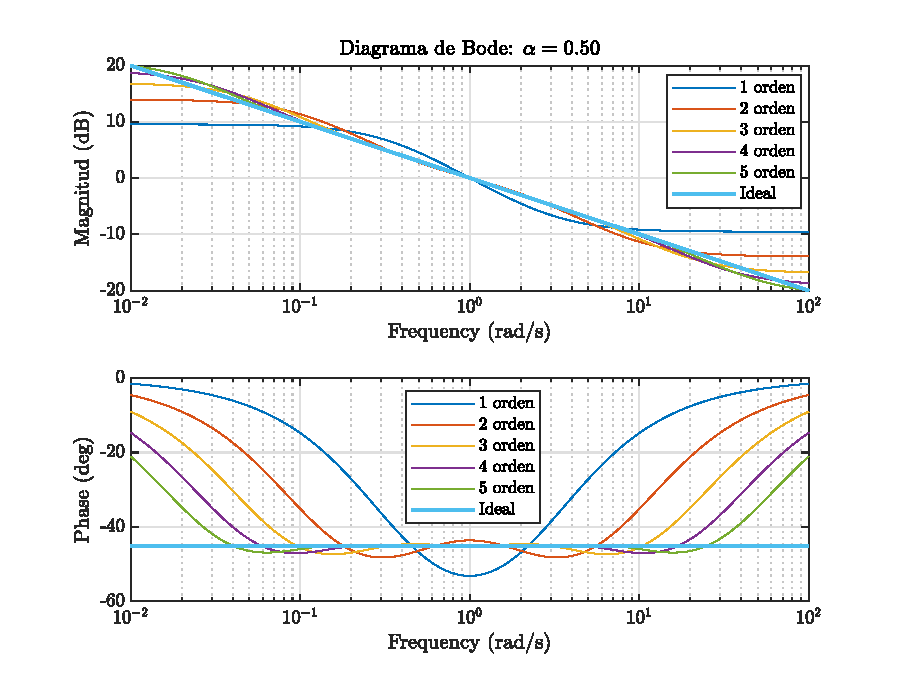
\includegraphics[width=12cm]{F1_bode_integrador_alpha05.eps}
	\end{figure}
	
	\subsection{Análisis de error de la CFE}
	Si variamos el orden $\alpha$ del integrador y el orden de la función de transferencia aproximada podemos notar que entre más pequeño sea $\alpha$ más se alejada la aproximación con respecto a un integrador fraccionario ideal, esto considerando el ancho de banda útil (ver Figuras \ref{fig:analisis_mag}, \ref{fig:analisis_fase}). Para cuantificar lo anterior existen dos tipos de errores de interés, el error sin normalizar y el error normalizado.
	
	El error en dB de la magnitud sin normalizar se puede calcular utilizando la siguiente ecuación:
	\begin{equation}
		\mathrm{error}_{\mathrm{dB}} = 20\log_{10} \left| \frac{H(j\omega)}{G(j\omega)} \right|
		\label{ec:error_sin_norm}
	\end{equation}
	donde $H(j\omega)$ es el integrador ideal $\frac{1}{s^{\alpha}}$ y $G(j\omega)$ es la función de transferencia aproximada del integrador utilizando CFE $ _{(c_{n})} \frac{1}{s^{\alpha}}$. 
	
	El error en grados de la fase sin normalizar se obtiene utilizando la siguiente ecuación:
	
	\begin{equation}
		\mathrm{error}_{\mathrm{deg}} = \phase{H(j\omega)} - \phase{G(j\omega)}
	\end{equation}
	
	Debido a que un integrador fraccionario ideal es en esencia un polo en el origen elevado a una potencia, este tiene un comportamiento de $-20 \alpha$ dB/década en magnitud y de $-90\alpha$ grados en fase \cite{CharlesAlexander2016}. Para normalizar el error este hecho resulta importante ya que la magnitud del integrador ideal en $0.1$ rad/seg para cualquier $\alpha$ siempre será $20 \alpha$ dB y para $10$ rad/seg de $-20 \alpha$ dB, de manera similar la fase permanece constante en $-90\alpha$ grados para cualquier $\alpha$.
	
	Entonces la ecuación para el error normalizado de magnitud es:
	
	\begin{equation}
		\mathrm{error}_{\mathrm{norm\,\,de\,\,mag}} = \cfrac{ 20\log_{10} \left| \frac{H(j\omega)}{G(j\omega)} \right| }{20 \alpha} = \cfrac{ \log_{10} \left| \frac{H(j\omega)}{G(j\omega)} \right| }{ \alpha}
	\end{equation}
	y la ecuación para el error normalizado de fase es:
	
	\begin{equation}
		\mathrm{error}_{\mathrm{norm\,\,de\,\,fase}} = \cfrac{\phase{H(j\omega)} - \phase{G(j\omega)}}{90\alpha}
	\end{equation}
	
	Para poder comparar los errores de manera precisa se debe calcular el valor absoluto de los errores para tener una medida de cuanto se aleja del integrador fraccionario ideal. En las Tablas \ref{tab:max_error_mag} y \ref{tab:max_error_fase} se muestran los errores absolutos máximos sin normalizar para la magnitud y la fase dependiente de $\alpha$ y el orden de la función de transferencia, estos datos se puede corroborar dirigiéndose a las gráficas de las Figuras \ref{fig:analisis_error_mag} y \ref{fig:analisis_error_fase}.
	
	\begin{table}[!hbp]                                 
	\centering            
	\caption{Máximo error absoluto de magnitud en dB variando $\alpha$ y orden de función de transferencia.}                           
	\label{tab:max_error_mag}                               
		\begin{tabular}{cccccc}
			\hline                                             
			$\,\,\,\,\bm{\alpha}$\textbf{/Orden} & \textbf{1$^{\mathrm{er}}$} & \textbf{2$^{\mathrm{do}}$} & \textbf{3$^{\mathrm{er}}$} & \textbf{4$^{\mathrm{to}}$} & \textbf{5$^{\mathrm{to}}$} \\                     
			\hline                                             
			0.1 & 0.4587 & 0.3333 & 0.2427 & 0.0620 & 0.0220 \\
			                                           
			0.2 & 0.8931 & 0.6524 & 0.4665 & 0.1172 & 0.0423 \\
			                                            
			0.3 & 1.2792 & 0.9426 & 0.6527 & 0.1596 & 0.0591 \\
			                                            
			0.4 & 1.5942 & 1.1889 & 0.7838 & 0.1848 & 0.0710 \\
			                                            
			0.5 & 1.8155 & 1.3748 & 0.8449 & 0.1904 & 0.0767 \\
			                                           
			0.6 & 1.9193 & 1.4807 & 0.8259 & 0.1767 & 0.0755 \\
			                                            
			0.7 & 1.8769 & 1.4676 & 0.7232 & 0.1458 & 0.0669 \\
			                                            
			0.8 & 1.6464 & 1.2410 & 0.5415 & 0.1021 & 0.0510 \\
			                                           
			0.9 & 1.1460 & 0.7507 & 0.2939 & 0.0513 & 0.0284 \\
			\hline                                             
		\end{tabular}                                                             
	\end{table}


	\begin{table}[!hbp]                                 
	\centering            
	\caption{Máximo error absoluto de fase en grados variando $\alpha$ y orden de función de transferencia.}                           
	\label{tab:max_error_fase}                               
		\begin{tabular}{cccccc}
			\hline                                             
			$\,\,\,\,\bm{\alpha}$\textbf{/Orden} & \textbf{1$^{\mathrm{er}}$} & \textbf{2$^{\mathrm{do}}$} & \textbf{3$^{\mathrm{er}}$} & \textbf{4$^{\mathrm{to}}$} & \textbf{5$^{\mathrm{to}}$} \\                     
			\hline                                             
			0.1 & 6.7092 & 2.8727 & 0.6548 & 0.5632 & 0.2796 \\ 
			                                             
			0.2 & 13.2833 & 5.5250 & 1.2598 & 1.0838 & 0.5338 \\
			                                            
			0.3 & 19.5614 & 7.7297 & 1.7677 & 1.5208 & 0.7390 \\
			                                              
			0.4 & 25.3200 & 9.2514 & 2.1362 & 1.8358 & 0.8760 \\
			                                            
			0.5 & 30.2099 & 9.8632 & 2.3294 & 1.9960 & 0.9311 \\
			                                             
			0.6 & 33.6307 & 9.3936 & 2.3198 & 1.9760 & 0.8975 \\
			                                             
			0.7 & 34.4722 & 7.8155 & 2.0880 & 1.7611 & 0.7756 \\
			                                             
			0.8 & 30.6494 & 5.3543 & 1.6237 & 1.3492 & 0.5739 \\
			                                             
			0.9 & 19.0601 & 2.5243 & 0.9255 & 0.7528 & 0.3080 \\
			\hline                                             
		\end{tabular}                                                             
	\end{table}

	A simple vista se podría creer que el error máximo aumenta conforme aumenta $\alpha$, no obstante esto es falso debido a que no se esta teniendo en cuenta la escala de la gráfica y por lo tanto las Tablas \ref{tab:max_error_mag} y \ref{tab:max_error_fase} únicamente nos dan información del total de error y no del porcentaje. Para tomar en cuenta la escala es necesario normalizar el error y de mismo modo calcular el valor absoluto de este. Las gráficas de la respuesta de magnitud y fase normalizadas se pueden encontrar en las Figuras \ref{fig:analisis_mag_norm} y \ref{fig:analisis_fase_norm}, y las gráficas de los errores normalizados en las Figuras \ref{fig:analisis_error_mag_norm} y \ref{fig:analisis_error_fase_norm}.
	
	En las Tablas \ref{tab:max_error_mag_norm} y \ref{tab:max_error_fase_norm} se muestran los porcentajes del máximo error absoluto normalizados para la magnitud y la fase. Haciendo un análisis de estas tablas se puede llegar a la conclusión de que en efecto \textbf{el porcentaje de error es mayor cuanto más pequeño sea $\bm{\alpha}$} y esto es de gran interés para poder generar reglas de diseño en la implementación de circuitos integradores fraccionarios.

	\begin{table}[!hbp]                                 
	\centering            
	\caption{Máximo error absoluto de magnitud normalizado en \% variando $\alpha$ y orden de función de transferencia.}                           
	\label{tab:max_error_mag_norm}                               
		\begin{tabular}{cccccc}
			\hline                                             
			$\,\,\,\,\bm{\alpha}$\textbf{/Orden} & \textbf{1$^{\mathrm{er}}$} & \textbf{2$^{\mathrm{do}}$} & \textbf{3$^{\mathrm{er}}$} & \textbf{4$^{\mathrm{to}}$} & \textbf{5$^{\mathrm{to}}$} \\                     
			\hline                                             
			0.1 & 22.9364 & 16.6661 & 12.1365 & 3.1006 & 1.1022 \\
			                                               
			0.2 & 22.3267 & 16.3092 & 11.6624 & 2.9299 & 1.0576 \\
			                                                
			0.3 & 21.3204 & 15.7107 & 10.8780 & 2.6595 & 0.9850 \\
			                                               
			0.4 & 19.9281 & 14.8618 & 9.7974 & 2.3094 & 0.8869 \\ 
			                                               
			0.5 & 18.1555 & 13.7481 & 8.4493 & 1.9044 & 0.7669 \\ 
			                                                
			0.6 & 15.9941 & 12.3390 & 6.8823 & 1.4724 & 0.6290 \\ 
			                                              
			0.7 & 13.4063 & 10.4826 & 5.1656 & 1.0415 & 0.4779 \\ 
			                                              
			0.8 & 10.2900 & 7.7565 & 3.3847 & 0.6380 & 0.3190 \\  
			                                             
			0.9 & 6.3665 & 4.1706 & 1.6328 & 0.2848 & 0.1578 \\  
			\hline                                             
		\end{tabular}                                                             
	\end{table}


	\begin{table}[!hbp]                                 
	\centering            
	\caption{Máximo error absoluto de fase normalizado en \% variando $\alpha$ y orden de función de transferencia.}                           
	\label{tab:max_error_fase_norm}                               
		\begin{tabular}{cccccc}
			\hline                                             
			$\,\,\,\,\bm{\alpha}$\textbf{/Orden} & \textbf{1$^{\mathrm{er}}$} & \textbf{2$^{\mathrm{do}}$} & \textbf{3$^{\mathrm{er}}$} & \textbf{4$^{\mathrm{to}}$} & \textbf{5$^{\mathrm{to}}$} \\                     
			\hline                                             
			0.1 & 74.5462 & 31.9184 & 7.2756 & 6.2574 & 3.1070 \\
			                                             
			0.2 & 73.7962 & 30.6945 & 6.9988 & 6.0212 & 2.9653 \\
			                                             
			0.3 & 72.4496 & 28.6284 & 6.5472 & 5.6324 & 2.7370 \\
			                                             
			0.4 & 70.3334 & 25.6983 & 5.9338 & 5.0995 & 2.4334 \\
			                                             
			0.5 & 67.1331 & 21.9182 & 5.1765 & 4.4355 & 2.0692 \\
			                                              
			0.6 & 62.2790 & 17.3955 & 4.2958 & 3.6593 & 1.6620 \\
			                                              
			0.7 & 54.7178 & 12.4056 & 3.3143 & 2.7954 & 1.2312 \\
			                                               
			0.8 & 42.5686 & 7.4365 & 2.2552 & 1.8739 & 0.7971 \\ 
			                                              
			0.9 & 23.5310 & 3.1165 & 1.1426 & 0.9293 & 0.3802 \\ 
			\hline                                             
		\end{tabular}                                                             
	\end{table}

	Dado que el máximo error ocurre en un rango de frecuencias muy corto es recomendable conocer de igual manera el error promedio, en las Tablas \ref{tab:prom_error_mag_norm} y \ref{tab:prom_error_fase_norm} se muestra el error promedio normalizado, este tipo de error presenta el mismo efecto de porcentaje de error con respecto a $\alpha$ que el máximo error normalizado. De los datos de las tablas podemos resaltar que en cuanto a magnitud, utilizar una aproximación de segundo orden en lugar de una de primer orden disminuye el error un 5.86 \% para $\alpha = 0.1$ y un 2.96 \% para $\alpha = 0.9$, en fase el cambio es aún mas notorio, el error disminuye un 26.71 \% para $\alpha = 0.1$ y un 5.61 \% para $\alpha = 0.9$. No obstante si nos detenemos a pensar detenidamente, con un $\alpha=0.9$ y una aproximación de primer orden el error promedio es de 4.22 \% en magnitud y de 6.55 \% en fase, el cual, para algunas aplicaciones puede resultar aceptable y cambiar por una aproximación de segundo orden no representaría una gran mejora, lo contrario ocurre con un $\alpha=0.1$, al cambiar a una aproximación de segundo orden el error se reduce significativamente, aproximadamente a la mitad en magnitud y a un cuarto en fase, en este caso en definitiva vale la pena cambiar.

	\begin{table}[!ht]                                 
	\centering            
	\caption{Promedio de error absoluto de magnitud normalizado en \% variando $\alpha$ y orden de función de transferencia.}                           
	\label{tab:prom_error_mag_norm}                               
		\begin{tabular}{cccccc}
			\hline                                             
			$\,\,\,\,\bm{\alpha}$\textbf{/Orden} & \textbf{1$^{\mathrm{er}}$} & \textbf{2$^{\mathrm{do}}$} & \textbf{3$^{\mathrm{er}}$} & \textbf{4$^{\mathrm{to}}$} & \textbf{5$^{\mathrm{to}}$} \\                     
			\hline                                             
			0.1 & 13.4397 & 7.5755 & 2.4058 & 0.5407 & 0.2754 \\
			                                         
			0.2 & 13.1089 & 7.3398 & 2.2960 & 0.5155 & 0.2639 \\
			                                              
			0.3 & 12.5614 & 6.9432 & 2.1189 & 0.4751 & 0.2454 \\
			                                            
			0.4 & 11.8034 & 6.3812 & 1.8827 & 0.4217 & 0.2203 \\
			                                            
			0.5 & 10.8454 & 5.6502 & 1.5991 & 0.3580 & 0.1897 \\
			                                           
			0.6 & 9.7075 & 4.7507 & 1.2822 & 0.2875 & 0.1548 \\ 
			                                         
			0.7 & 8.4275 & 3.6945 & 0.9478 & 0.2133 & 0.1168 \\ 
			                                              
			0.8 & 6.8606 & 2.5119 & 0.6123 & 0.1387 & 0.0772 \\ 
			                                             
			0.9 & 4.2249 & 1.2563 & 0.2916 & 0.0667 & 0.0377 \\ 
			\hline                                             
		\end{tabular}                                                             
	\end{table}


	\begin{table}[!ht]                                 
	\centering            
	\caption{Promedio error absoluto de fase normalizado en \% variando $\alpha$ y orden de función de transferencia.}                           
	\label{tab:prom_error_fase_norm}                               
		\begin{tabular}{cccccc}
			\hline                                             
			$\,\,\,\,\bm{\alpha}$\textbf{/Orden} & \textbf{1$^{\mathrm{er}}$} & \textbf{2$^{\mathrm{do}}$} & \textbf{3$^{\mathrm{er}}$} & \textbf{4$^{\mathrm{to}}$} & \textbf{5$^{\mathrm{to}}$} \\                     
			\hline                                             
			0.1 & 34.9335 & 8.2174 & 2.6873 & 1.3313 & 0.3667 \\
			                                              
			0.2 & 34.0430 & 7.8450 & 2.5975 & 1.2737 & 0.3498 \\
			                                           
			0.3 & 32.5319 & 7.2389 & 2.4512 & 1.1805 & 0.3226 \\
			                                              
			0.4 & 30.3547 & 6.4219 & 2.2473 & 1.0556 & 0.2864 \\
			                                            
			0.5 & 27.4424 & 5.4308 & 1.9840 & 0.9042 & 0.2431 \\
			                                          
			0.6 & 23.6947 & 4.3175 & 1.6640 & 0.7329 & 0.1948 \\
			                                             
			0.7 & 18.9857 & 3.1492 & 1.2933 & 0.5488 & 0.1439 \\
			                                           
			0.8 & 13.2152 & 2.0009 & 0.8821 & 0.3598 & 0.0929 \\
			                                              
			0.9 & 6.5510 & 0.9388 & 0.4450 & 0.1742 & 0.0441 \\ 
			\hline                                             
		\end{tabular}                                                             
	\end{table}


	De ser necesario para convertir el error de magnitud normalizado de \% a dB se utiliza la siguiente ecuación:
	
	\begin{equation}
		\mathrm{error}_{\mathrm{dB}} =  20 \alpha \cdot \left( \frac{\%_{\mathrm{error\,\,mag}}}{100} \right)
	\end{equation}
	y para el error de fase normalizado de \% a grados:
	
	\begin{equation}
		\mathrm{error}_{\mathrm{deg}} = 90 \alpha \cdot \left( \frac{\%_{\mathrm{error\,\,fase}}}{100} \right) 
	\end{equation}
	                                                                 
	\section{Escalamiento en frecuencia}
	
	Debido a que el ancho de banda del integrador fraccionario utilizando la aproximación de CFE es de aproximadamente dos décadas y se encuentra en un rango de frecuencia muy bajo, de 0.1 rad/s hasta 10 rad/s, el cual es un rango poco útil en aplicaciones reales, es necesario escalar la respuesta en frecuencia.
	
	El escalamiento en frecuencia es el proceso de correr la respuesta en frecuencia de una red por arriba o por abajo del eje de frecuencia mientras  se mantiene igual la impedancia \cite{CharlesAlexander2016}.
	
	El escalamiento de frecuencia se consigue multiplicando ésta por un factor de escalamiento $k_{f}$ mientras se mantiene la impedancia igual. Si consideramos $p$ la variable de frecuencia compleja actual y $s$ la escalada, el proceso de escalamiento se define por la siguiente relación \cite{Allen1980}:
	
	\begin{equation}
		s = k_{f} p
		\label{ec:escalamiento}
	\end{equation}
	la ecuación (\ref{ec:escalamiento}) también se puede ver de la siguiente manera:
	
	\begin{equation}
		k_{f} = \frac{s}{p} = \frac{j \omega^{'}}{j \omega} = \frac{\omega^{'}}{\omega}
	\end{equation}
	donde $\omega^{'}$ es la frecuencia escalada y $\omega$ es la frecuencia actual de referencia.
	
	Para entender de mejor manera el escalamiento en frecuencia estudiemos el siguiente ejemplo, consideremos la siguiente función de transferencia:
	
	\begin{equation}
		N(p) = \frac{20p}{p^{2} + 12p + 20}
	\label{ec:esc_ejem}
	\end{equation}
	la cual corta el eje de la frecuencia en 0.1 rad/s y 200 rad/s. Si deseamos que la respuesta en magnitud permanezca idéntica pero desplazada a la derecha en un factor de cien, es decir, que las frecuencias escaladas corten el eje de frecuencia en 10 rad/s y 20k rad/s, entonces $k_{f} = \frac{10}{0.1} = 100$, sustituyendo la ecuación (\ref{ec:escalamiento}) en (\ref{ec:esc_ejem}):

	\begin{equation}
		N(s) = \frac{200sk_{f}^{-1}}{s^{2}k^{-2}_{f} + 12sk^{-1}_{f} + 20} = \frac{200k_{f}s}{s^{2} + 12 k_{f} s + 20 k^{2}_{f}}
	\end{equation}
	entonces la función de transferencia escalada resulta:

	\begin{equation}
		N(s)  = \frac{200(100)s}{s^{2} + 12(100)s + 20(100)^{2}}
	\end{equation}
	
	En la Figura \ref{fig:F10_bode_escalamiento} se muestra el resultado de aplicar el escalamiento en frecuencia a la ecuación \ref{ec:esc_ejem}. Si se desea aplicar el escalamiento en Hz, simplemente se tiene que tener en consideración el factor de conversión, como ejemplo, si se desea que las frecuencias que corten el eje de la frecuencia sean 0.1 Hz y 200 Hz entonces:
	
	\begin{equation}
		k_{f} = \frac{0.1 \,\,\mathrm{Hz} \cdot \frac{2 \pi \,\,\mathrm{rad/s}}{1 \,\,\mathrm{Hz}}}{0.1 \,\,\mathrm{rad/s}} = 2 \pi
	\end{equation}
	
	\begin{figure}[hbtp]
		\caption{Diagrama de bode comparativo de función de transferencia escalada.} 
		\label{fig:F10_bode_escalamiento}
		\centering
		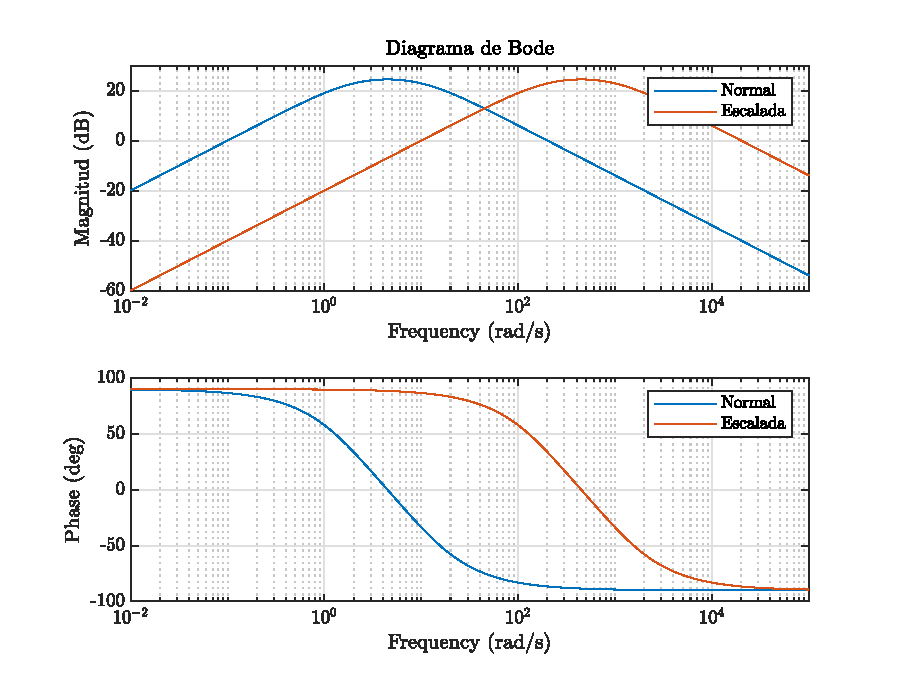
\includegraphics[width=12cm]{F10_bode_escalamiento.eps}
	\end{figure}
	
	Esta metodología se puede aplicar a cualquier función de transferencia y tiene la ventaja de solo ser necesario modificar el factor de escalamiento $k_{f}$ una vez obtenida la expresión escalada.
	\section{Teoría de filtros}
	
	Las funciones de transferencia obtenidas de la CFE pueden ser llevadas al mundo real utilizando filtros, ya sean activos, pasivos, de primer orden (bilineales), segundo orden (bicuadraticos) o de ordenes superiores usando una combinaciones de ambos. Por esta razón es de interés estudiar brevemente la teoría de filtros, tener presente las estructuras matemáticas más comunes en el diseño de filtros y sus principales características.
	
		\subsection{Filtros de primer orden}
	
	La función de transferencia general de primer orden esta dada por la siguiente ecuación:
	
	\begin{equation}
		T(s) = \frac{a_{1} s + a_{0} }{s + \omega_{0}}
		\label{ec:bilineal_general}
	\end{equation}
	esta función de transferencia bilineal se caracteriza por tener un polo en $s = - \omega_{0}$, un cero en $s = -\frac{a_{0}}{a_{1}}$ y una ganancia de alta frecuencia que tiende a $a_{1}$. Los coeficientes del numerador, $a_{0}$ y $a_{1}$, determinan el tipo de filtro, ya sea pasabajas (LP), pasaaltas (HP), pasatodas (AP) o general. La realización activa provee considerablemente más versatilidad que su contra parte pasiva, en muchos casos la ganancia puede ser ajustada a un valor deseado, y algunos parámetros de las funciones de transferencia también sin afectar otros. La impedancia de salida de los circuitos activos es muy baja, haciendo que la colocación en cascada sea muy fácil. Sin embargo, los amplificadores operacionales limitan la operación a altas frecuencias de los circuitos activos \cite{Sedra2015}. En la Figura \ref{fig:primer_orden_plano_s} se muestra la ubicación del polo y el cero de los diferentes tipos de filtros que se pueden formar para la configuración bilineal.
	
	\begin{figure}[!ht]
	\centering   
	\caption{Singularidades de filtros de primer orden en el plano $s$.}
	\label{fig:primer_orden_plano_s}
		\begin{subfigure}{0.48\textwidth}
			\centering   
			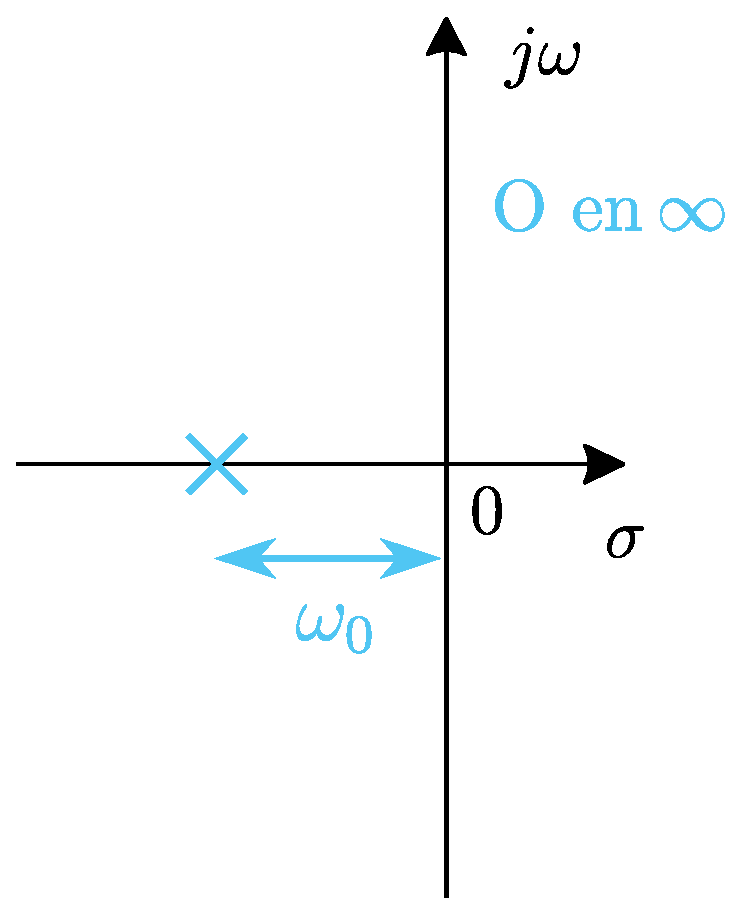
\includegraphics[width=0.9\linewidth, width=5cm]{U1_pasabajas.eps} 
			\caption{Pasabajas.}
			\label{fig:U1_pasabajas}
		\end{subfigure}
		\begin{subfigure}{0.48\textwidth}
			\centering   
			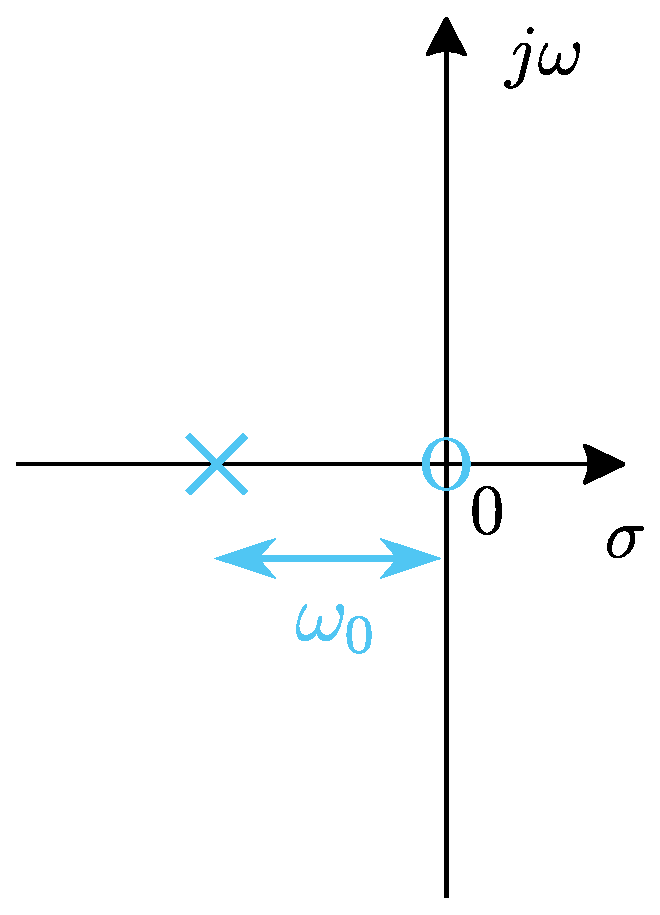
\includegraphics[width=0.9\linewidth, width=4.3cm]{U2_pasaaltas.eps}
			\caption{Pasaaltas.}
			\label{fig:U2_pasaaltas}
		\end{subfigure}
		\begin{subfigure}{0.48\textwidth}
			\centering   
			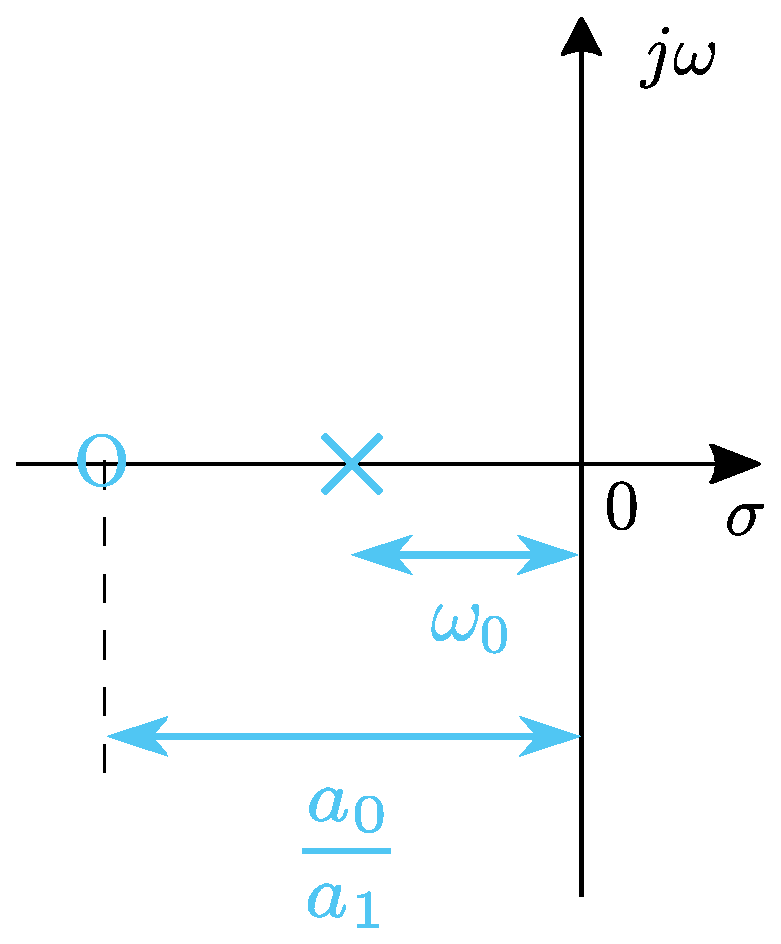
\includegraphics[width=0.9\linewidth, width=5cm]{U3_general.eps} 
			\caption{General.}
			\label{fig:U3_general}
		\end{subfigure}
		\begin{subfigure}{0.48\textwidth}
			\centering   
			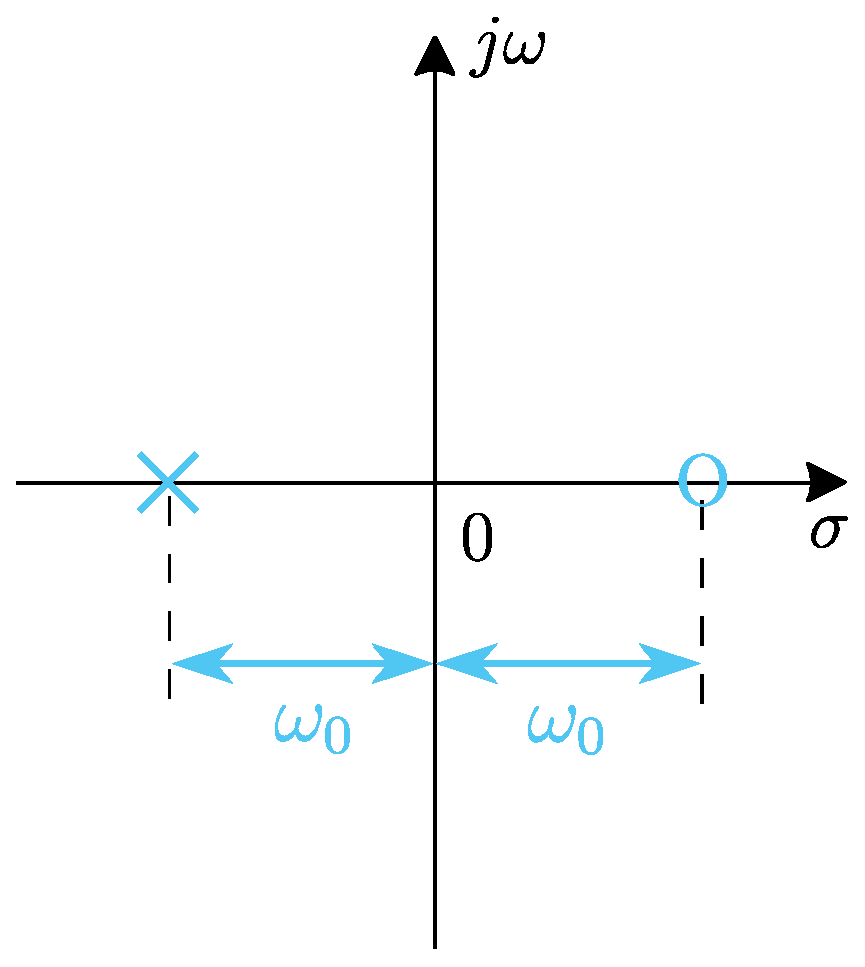
\includegraphics[width=0.9\linewidth, width=5.5cm]{U4_allpass.eps}
			\caption{Pasatodas.}
			\label{fig:U4_allpass}
		\end{subfigure}
	\end{figure}
	
	Diferentes tipos de filtros nacen de ubicar el cero de la función de transferencia bilineal general (\ref{ec:bilineal_general}) en distintos lugares, un cero en el infinito genera un filtro pasabajas de primer orden, y un cero en el origen un filtro pasaaltas. Un cero colocado simétricamente relativo al eje $j\omega$ genera un pasatodas. Las ecuaciones básicas de los filtros de primer orden son las siguientes:
	
	
	\begin{itemize}
		\item Pasabajas (LP)
		\begin{equation}
			T(s) = \frac{a_{0}}{s + \omega_{0}}
		\end{equation}
	
		\item Pasaaltas (HP)
		\begin{equation}
			T(s) = \frac{a_{1}s}{s + \omega_{0}}
		\end{equation}
		
		\item Pasatodas (AP)
		\begin{equation}
			T(s) = -a_{1} \frac{s - \omega_{0}}{s + \omega_{0}}
		\end{equation}
	\end{itemize}
	
		\subsection{Filtros de segundo orden}
	
	La función de transferencia general de un filtro de segundo orden o bicuadrátrica se expresa en lo general en la forma estándar:
	
	\begin{equation}
		T(s) = \frac{a_{2} s^{2} + a_{1}s + a_{0}}{s^{2} + \left( \cfrac{ \omega_{0} }{Q} \right)s + \omega_{0}^{2}}
	\end{equation}
	donde $\omega_{0}$ y $Q$ determinan los polos de acuerdo a la siguiente ecuación:
	
	\begin{equation}
		p_{1,2} = - \frac{\omega_{0}}{2 Q} \pm j \omega_{0} \sqrt{1 - \left(   \frac{1}{4 Q^{2}}  \right) \,\,}
	\end{equation}
	al parámetro $\omega_{0}$ se le conoce como frecuencia de polo, y representa la distancia radial entre el origen y el polo en el plano complejo $s$. $Q$ es el factor de calidad de polo y determina la distancia de los polos desde el eje $j\omega$, una representación gráfica de estos parámetros se muestra en la Figura \ref{fig:F11_parametros_Q_w}, entre más grande sea el valor de $Q$, más cerca estarán los polos el eje $j\omega$, y la respuesta del filtro se vuelve más selectiva. Un valor infinito para $Q$ localiza a los polos sobre el eje $j\omega$ y puede producir oscilaciones sostenidas en la realización del circuito. Un valor negativo de $Q$ implica que los polos se encuentran en la mitad derecha del plano s, lo cual ciertamente produce oscilaciones.
	Los ceros del filtro de segundo orden están determinados por los coeficientes del numerador, $a_{0}$, $a_{1}$ y $a_{2}$, en otras palabras los coeficientes del numerador determinan el tipo de filtro de segundo orden \cite{Sedra2015}.
	
	Para un filtro pasabajas (LP) de segundo orden, los dos ceros están en $s = \infty$ y su respuesta de magnitud muestra un pico para $Q > \frac{1}{\sqrt{2}}$. Para un pasaaltas (HP) los ceros están en $s = 0$ y su respuesta de magnitud también muestra un pico para $Q > \frac{1}{\sqrt{2}}$. Para un pasabanda (BP) un cero esta en $s = \infty$ y el otro en $s = 0$, la respuesta de magnitud tiene un pico en $\omega = \omega_{0}$, por lo tanto, la frecuencia central del filtro pasabandas es igual a la frecuencia de polo $\omega_{0}$. La selectividad de del filtro pasabanda de segundo orden es usualmente medida por su ancho de banda de 3 dB. Este es la diferencia entre las dos frecuencias $\omega_{1}$ y $\omega_{2}$ en las cuales la respuesta de magnitud es 3 dB por debajo de su valor máximo el cual ocurre en $\omega_{0}$. La ecuación que describe a las frecuencias $\omega_{1},\omega_{2}$ es la siguiente:
	
	\begin{equation}
		\omega_{1},\omega_{2} = \omega_{0} \sqrt{1 + \left( \frac{1}{4 Q^{2}} \right)}  \pm \frac{\omega_{0}}{2 Q}
	\end{equation}
	Entonces el ancho de banda $BW$ se define como:
	
	\begin{equation}
	BW = \omega_{2} - \omega_{1} = \frac{\omega_{0}}{Q}
	\end{equation}
	
	
	\begin{figure}[hbtp]
		\caption{Definición de los parámetros $\omega_{0}$ y $Q$ de un par de polos conjugados.} 
		\label{fig:F11_parametros_Q_w}
		\centering
		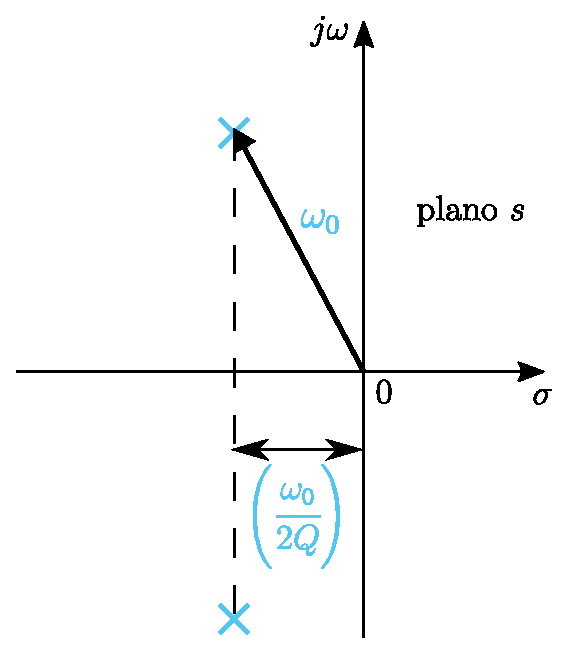
\includegraphics[width=5cm]{F11_parametros_Q_w.eps}
	\end{figure}
	
	Las ecuaciones básicas de filtros de segundo orden son las siguientes:
	\begin{itemize}
	\item Pasabajas (LP)
	\begin{equation}
	T(s) = \frac{a_{0}}{s^{2} + \cfrac{\omega_{0}}{Q} s + \omega_{0}^{2}}
	\end{equation}
	
	\item Pasaaltas (HP)
	\begin{equation}
	T(s) = \frac{a_{2} s^{2}}{s^{2} + \cfrac{\omega_{0}}{Q} s + \omega_{0}^{2}}
	\end{equation}
	
	\item Pasabandas (BP)
	\begin{equation}
	T(s) = \frac{a_{1} s}{s^{2} + \cfrac{\omega_{0}}{Q} s + \omega_{0}^{2}}
	\end{equation}
	
	\item Pasatodas (AP)
	\begin{equation}
	T(s) = a_{2} \frac{s^{2} - \cfrac{\omega_{o}}{Q}s + \omega_{0}^{2} }{s^{2} + \cfrac{\omega_{0}}{Q} s + \omega_{0}^{2}}
	\end{equation}
	\end{itemize}
	
	En la Figura \ref{fig:segundo_orden_plano_s} se muestran las singularidades de los filtros más comunes de segundo orden.
	\begin{figure}[!ht]
	\centering   
	\caption{Singularidades de filtros de segundo orden en el plano $s$.}
	\label{fig:segundo_orden_plano_s}
		\begin{subfigure}{0.48\textwidth}
			\centering   
			\includegraphics[width=0.9\linewidth, width=6cm]{V1_pasabajas_segundo.eps} 
			\caption{Pasabajas.}
			\label{fig:V1_pasabajas_segundo}
		\end{subfigure}
		\begin{subfigure}{0.48\textwidth}
			\centering   
			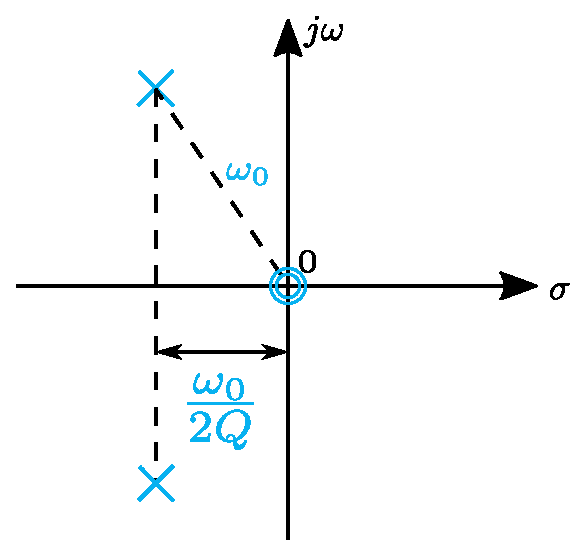
\includegraphics[width=0.9\linewidth, width=6cm]{V2_pasaaltas_segundo.eps}
			\caption{Pasaaltas.}
			\label{fig:V2_pasaaltas_segundo}
		\end{subfigure}
		\begin{subfigure}{0.48\textwidth}
			\centering   
			\includegraphics[width=0.9\linewidth, width=6cm]{V3_pasabanda_segundo.eps} 
			\caption{Pasabanda.}
			\label{fig:V3_pasabanda_segundo}
		\end{subfigure}
		\begin{subfigure}{0.48\textwidth}
			\centering   
			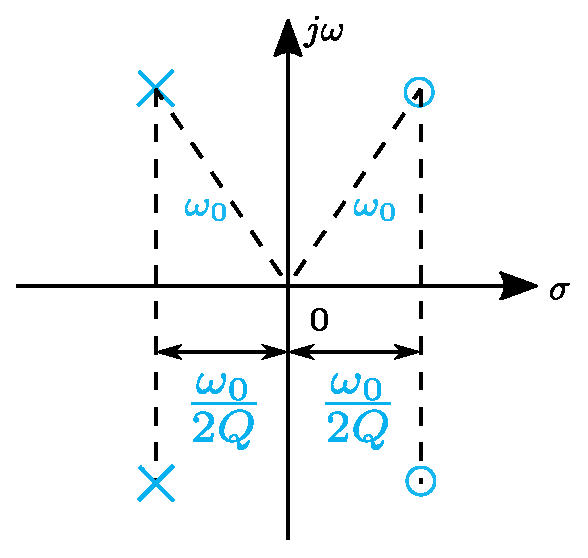
\includegraphics[width=0.9\linewidth, width=6cm]{V4_pasatodas_segundo.eps}
			\caption{Pasatodas.}
			\label{fig:V4_pasatodas_segundo}
		\end{subfigure}
	\end{figure}
	
	Las estructuras matemáticas estudiadas en este sección servirán como herramientas en secciones posteriores. 
	\chapter{Implementación }

	\section{AnadigmDesigner2}



\appendix
	\chapter{Códigos}

\lstinputlisting[style = MATLAB, caption =  Función syms2tf, label = cod:syms2tf]{codigos/syms2tf.m}

\lstinputlisting[style = MATLAB, caption =  Función cfetf, label = cod:cfetf]{codigos/cfetf.m}

\lstinputlisting[style = MATLAB, caption =  Función A10\_{}calculo\_{}valores\_{}FilterBilienar, label = cod:A10_calculo_valores_FilterBilienar]{codigos/A10_calculo_valores_FilterBilienar.m}

\lstinputlisting[style = MATLAB, caption =  Función A11\_{}rango\_{}de\_{}frecuencias\_{}absolutas\_{}FilterBilinear, label = cod:A11_rango_de_frecuencias_absolutas_FilterBilinear]{codigos/A11_rango_de_frecuencias_absolutas_FilterBilinear.m}

\lstinputlisting[style = MATLAB, caption =  Función A12\_{}grafica\_{}analisis\_{}de\_{}frecuencias\_{}FilterBilinear, label = cod:A12_grafica_analisis_de_frecuencias_FilterBilinear]{codigos/A12_grafica_analisis_de_frecuencias_FilterBilinear.m}

\lstinputlisting[style = MATLAB, caption =  Función B10\_{}calculo\_{}valores\_{}suma\_{}filtros, label = cod:B10_calculo_valores_suma_filtros]{codigos/B10_calculo_valores_suma_filtros.m}

	\include{Ap_B}
	
	Cita 1 \cite{Petras2011}
	Cita 2 \cite{Petras2019}
	Cita 3 \cite{Olds2009}
	Cita 4 \cite{Li2018}
	Cita 5 \cite{Krishna2008}
	Cita 6 \cite{Krishna2011}
	

\backmatter

\bibliographystyle{ieeetr}
\bibliography{bibliografia}

\end{document}